% Created with jtex v.1.0.20
% \newcommand{\secondLanguage}{icelandic} 			% if a second language is used, add it here
% \documentclass[draft, {\secondLanguage}, english]{volcanica-template}
\documentclass[draft, english]{volcanica-template}
\nonstopmode									% can toggle to see compilation warnings
% Please choose between Research article, Report, Review, or Methods.
% Details about different article types are available at:
% https://www.jvolcanica.org/ojs/index.php/volcanica/about/submissions
\newcommand{\ArticleType}{Report}



%------------------------------------------------------------
%  Article details go here
%------------------------------------------------------------
\newcommand{\Title}{How to MyST, without being mystified} 	% Manuscript title goes here.
\newcommand{\shortTitle}{How to MyST} 		% Short title for header goes here, less than 60 characters.
\newcommand{\Author}{Alberto Durán Pérez\xspace}    	% First author goes here.

%------------------------------------------------------------
%  Author details go here
%------------------------------------------------------------
\author[{{\affiliation{1}\affiliation{2}}}]
{\orcidaffil{0000-0002-7859-8394}~Alberto Durán Pérez \Email{aduranperez@freimartinsarmiento.com}}

%------------------------------------------------------------
%  Affiliations
%------------------------------------------------------------
\affil[{{\affiliation{1}}}]{IES Frei Martín Sarmiento}
\affil[{{\affiliation{2}}}]{Departamento de Tecnología}

%------------------------------------------------------------
%  BIBLIOGRAPHY FILE
%------------------------------------------------------------
% \addbibresource{bib-file.bib} % add the name of the bibliography file here

%------------------------------------------------------------
%  Start of Document
%------------------------------------------------------------
\begin{document}

%------------------------------------------------------------
%  Abstract(s) and Keywords
%------------------------------------------------------------
% If there is a second-language abstract, it goes between the square brackets [].
% Make sure you have included the correct language in line 1, above.
% If no second abstract, ensure there is no space between the square brackets [].
\FrontMatter{Google Sheets es una aplicación de hoja de cálculo gratuita y basada en la web provista por Google Drive. Está diseñada para la colaboración en tiempo real, permitiendo que múltiples usuarios editen simultáneamente. Su estructura básica se define por la Ce  lda, Fila y Columna, y los formatos básicos aseguran la legibilidad, incluyendo el formato Moneda (ej. €) y el uso de bordes.
El procesamiento de datos utiliza Fórmulas (expresiones que comienzan con =) y operadores básicos (suma, división, etc.). Las Funciones pre-construidas clave incluyen SUMA, PROMEDIO (AVERAGE), MÁXIMO (MAX) y MÍNIMO (MIN).
La lógica condicional se gestiona mediante la Referencia Absoluta (\$) para fijar valores (ej. un Extra de 0,5 o el IVA del 21,00\%), y la Función SI (IF), que automatiza decisiones (ej. mostrar Aprobado o Suspenso). El Formato Condicional aplica estilos automáticamente (ej. notas $\geq$5 en verde).
Para el análisis avanzado, la función BUSCARV (VLOOKUP) busca valores (ej. la Densidad de Madrid: 841,17 hab/km\textsuperscript{2}). La función QUERY permite operaciones SQL-like. La herramienta Explore utiliza machine learning (IA) para sugerir gráficos y responder preguntas en lenguaje natural.
Finalmente, la automatización se facilita con Apps Script (entorno de bajo código para tareas como crear documentos y enviar correos electrónicos) y la integración con más de 8,000 aplicaciones (ej. Google Ads, Slack) a través de Zapier.}
[]%
{
\keywords{m}{y}{s}{t}{,}{ }{a}{r}{k}{d}{o}{w}{n}{p}{e}{-}{c}{i}	% add up to six keywords in curly braces {}
}

%------------------------------------------------------------
%  Maintext
%------------------------------------------------------------
\section{Bloque I: Estructura y Formatos Básicos de Google Sheets}

\subsection{1. ¿Qué es Google Sheets?}

\textbf{Google Sheets} (Hojas de Cálculo) es una aplicación de hoja de cálculo gratuita y basada en la web, provista por Google dentro del servicio \textbf{Google Drive}. Permite a los usuarios organizar, editar, analizar diferentes tipos de información, y es clave para el trabajo colaborativo, ya que múltiples usuarios pueden editar y dar formato a los archivos en tiempo real.

Una hoja de cálculo es el documento completo (o \textbf{Spreadsheet}) que contiene conjuntos de columnas y filas. Dentro de un documento, puede haber una o más \textbf{Worksheets} (hojas), que son conjuntos nombrados de filas y columnas.

\subsection{2. Vocabulario Estructural (Las Coordenadas)}

Para trabajar en Google Sheets, es esencial conocer los nombres de sus componentes principales, que forman una matriz o cuadrícula:

\bigskip\noindent
\begin{tabular}{p{\dimexpr 0.250\linewidth-2\tabcolsep}p{\dimexpr 0.250\linewidth-2\tabcolsep}p{\dimexpr 0.250\linewidth-2\tabcolsep}p{\dimexpr 0.250\linewidth-2\tabcolsep}}
\toprule
Concepto & Definición & Ejemplos (Basados en las Tareas) & Citas de Origen \\
\hline
\textbf{Celda} (Cell) & Es la unidad mínima y fundamental de información, o un solo punto de dato. Se identifica por la intersección de una columna y una fila. & B4, A9, E12, D5, F18. &  \\
\textbf{Columna} (Column) & Es la disposición vertical de celdas, identificada por letras (A, B, C...). & Colorear la \textbf{columna C} de color verde. &  \\
\textbf{Fila} (Row) & Es la disposición horizontal de celdas, identificada por números (1, 2, 3...). & Colorear la \textbf{fila 8} de color gris. &  \\
\textbf{Rango} (Range) & Es un conjunto rectangular de múltiples celdas adyacentes. Se define por las referencias de las celdas de las esquinas, separadas por dos puntos. & E3:G7 (rango de celdas coloreado de rosa). &  \\
\bottomrule
\end{tabular}

\bigskip

\begin{figure}[!htbp]
\centering
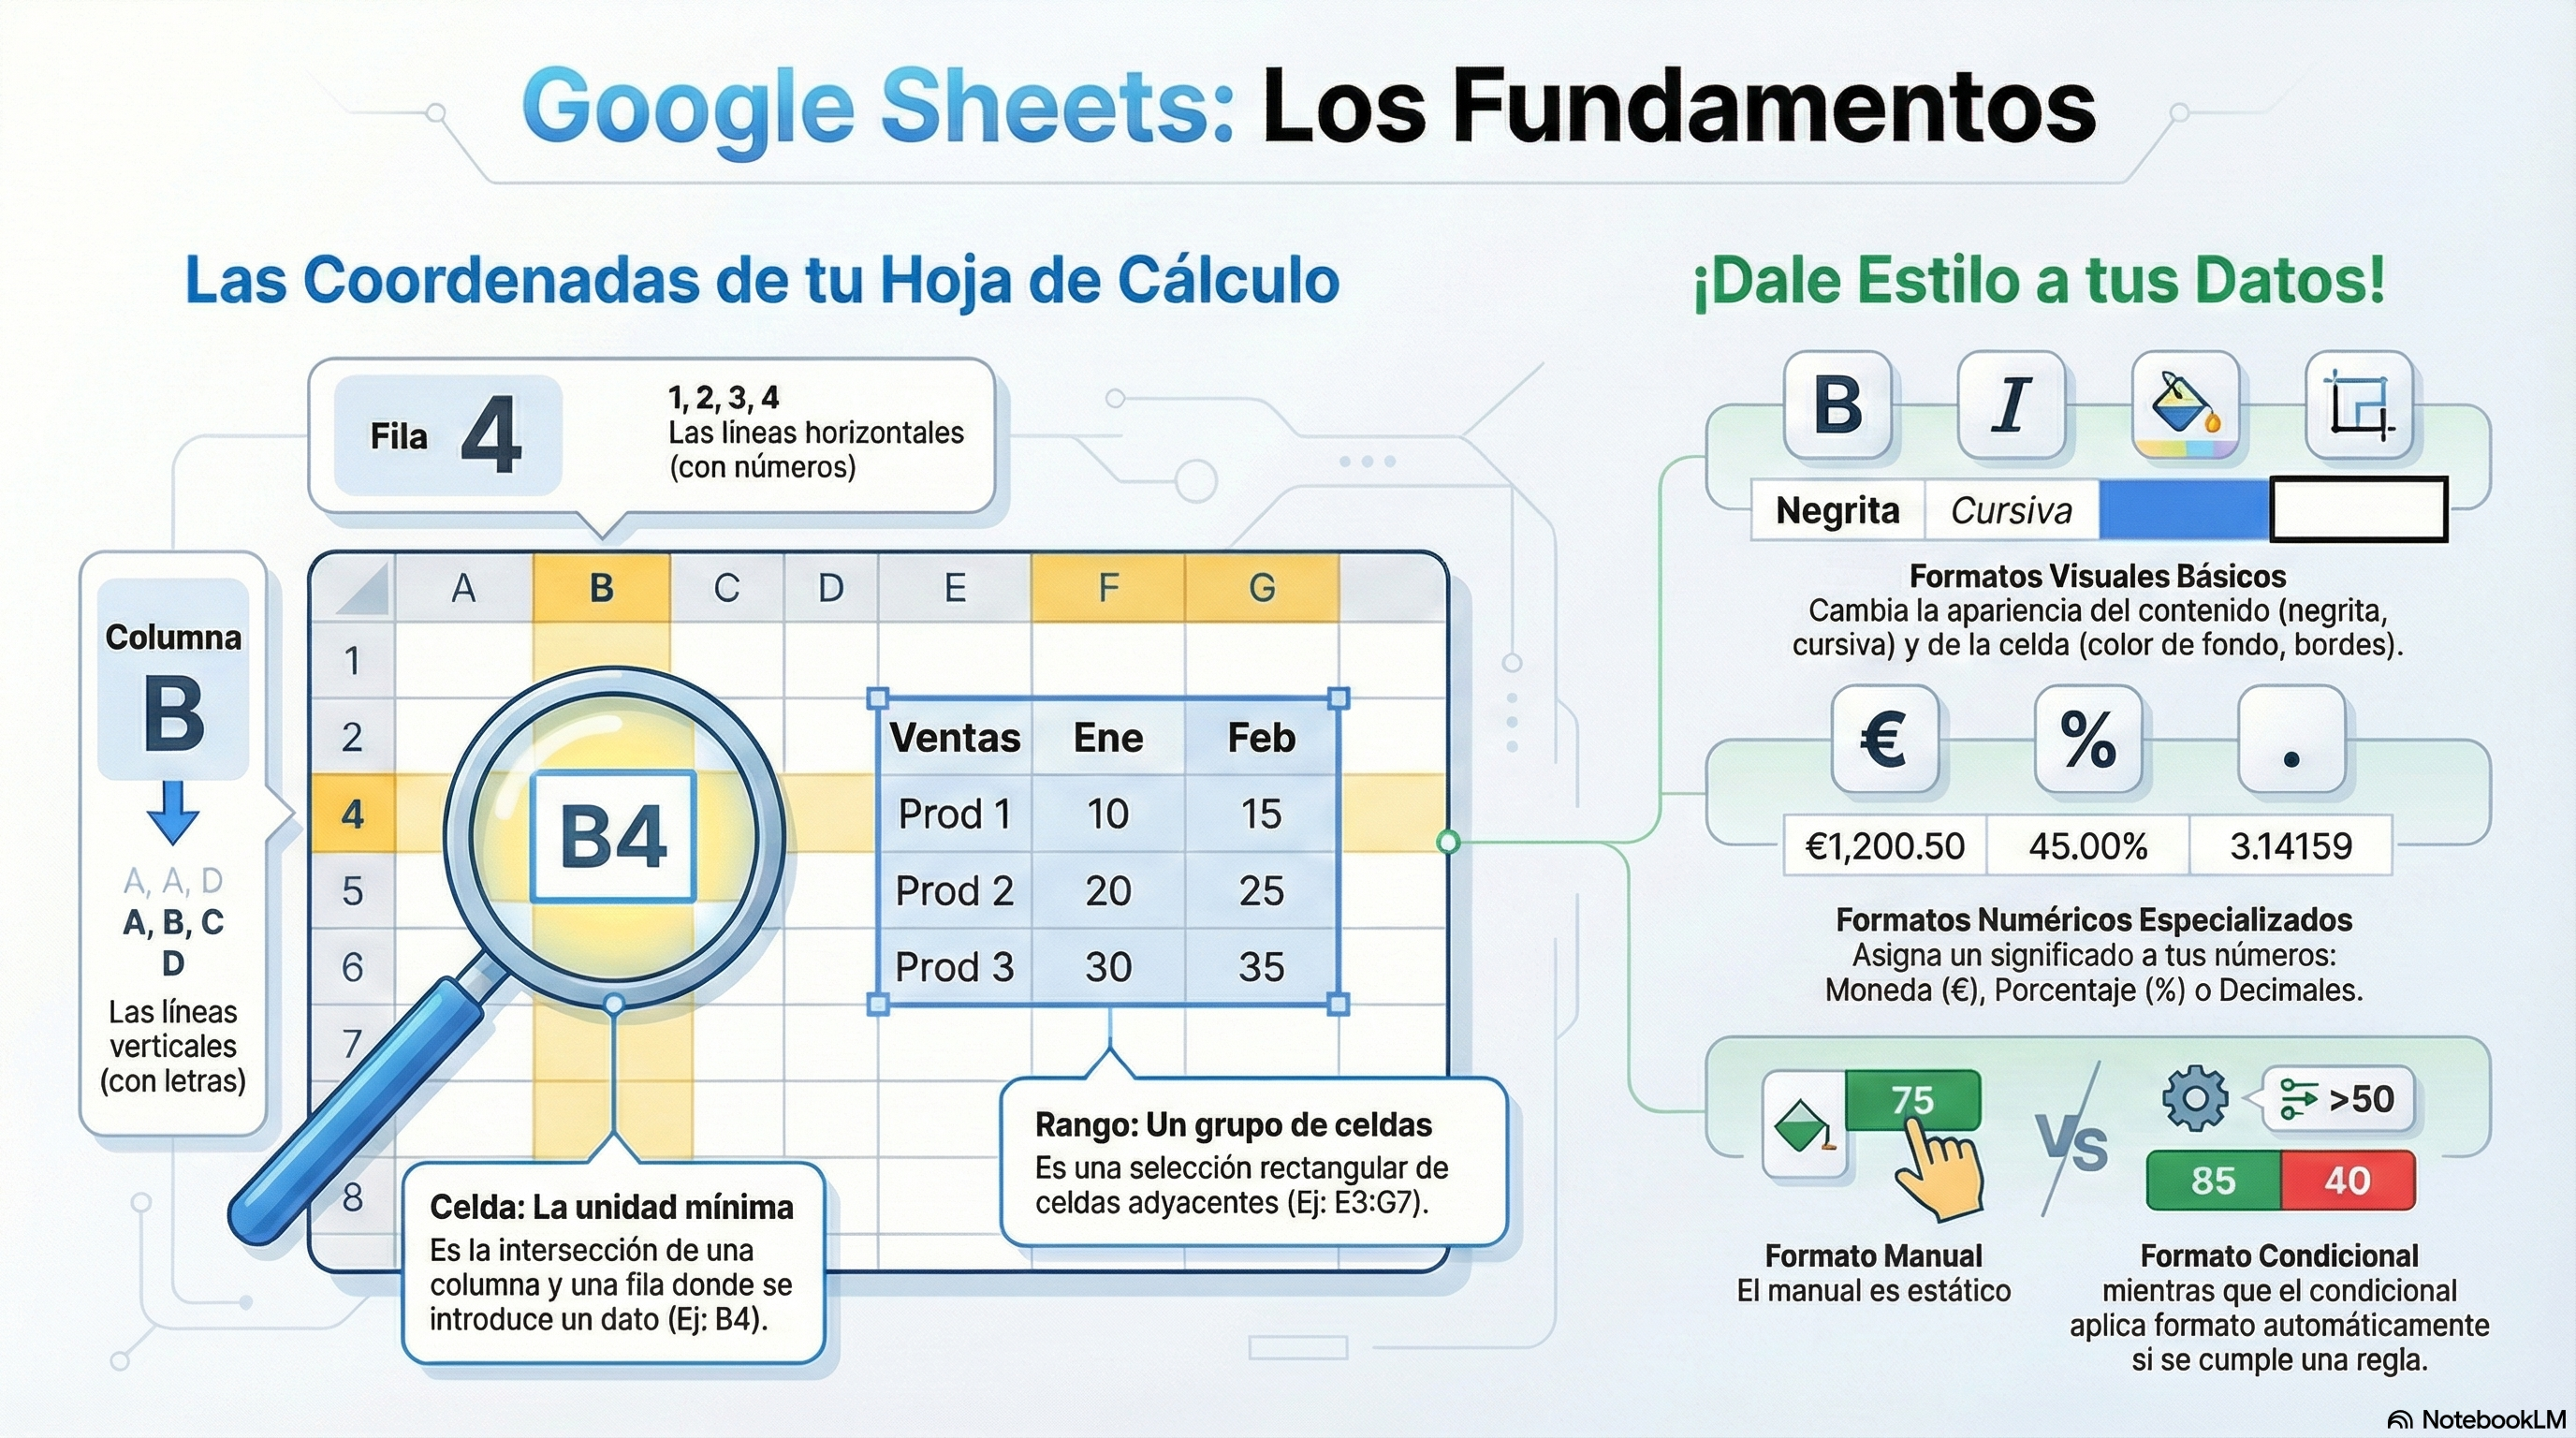
\includegraphics[width=0.7\linewidth]{files/bloque1-3aecd15cc5dfd16eb9127e655cc82eb9.png}
\caption[]{Fundamentos de Google Sheets.}
\label{fundamentos}
\end{figure}

\subsection{3. Entrada y Manipulación de Datos}

La forma en que se introducen y mueven los datos afecta la eficiencia del trabajo:

\begin{itemize}
\item \textbf{Entrada Básica:} Para añadir datos a una celda, simplemente se hace clic en ella y se escribe. Para facilitar la manipulación o el filtrado posterior, es una buena práctica que cada celda contenga solo un valor.
\item \textbf{Navegación:} Después de escribir en una celda, se puede presionar la tecla \texttt{Enter} o \texttt{return} para guardar el dato y mover el cursor al inicio de la \textbf{siguiente fila}. Alternativamente, se puede presionar \texttt{Tab} para guardar el dato y moverse una celda a la \textbf{derecha} dentro de la misma fila.
\item \textbf{El Puntero de Relleno (Fill Handle):} Es un pequeño signo de más (\texttt{+}) que aparece en la esquina inferior derecha de una celda seleccionada. Al arrastrar este puntero, se pueden copiar automáticamente datos, formatos o fórmulas a celdas adyacentes.
\end{itemize}

\subsection{4. Formatos de Celda (Estilo Manual)}

El formato manual permite modificar directamente la apariencia de los datos, mejorando la \textbf{presentación} y la \textbf{legibilidad}.

\subsubsection{A. Formato de Contenido (Texto y Números)}

\bigskip\noindent
\begin{tabular}{p{\dimexpr 0.250\linewidth-2\tabcolsep}p{\dimexpr 0.250\linewidth-2\tabcolsep}p{\dimexpr 0.250\linewidth-2\tabcolsep}p{\dimexpr 0.250\linewidth-2\tabcolsep}}
\toprule
Formato & Uso Práctico & Ejemplos de Contenido & Citas de Origen \\
\hline
\textbf{Estilo de Fuente} & Destacar información importante. Se utilizan: \textbf{Negrita}, \textbf{Subrayado} y \textbf{Cursiva}. & Escribir \textbf{6798} en \textbf{negrita}. Escribir \textbf{``Fotografía'' subrayada} en B10. Escribir el número \textbf{56} en \textbf{cursiva de color rojo}. &  \\
\textbf{Alineación} & Determinar la posición del contenido dentro de la celda. & \textbf{Centrar} la palabra \textbf{``Internet''} en la celda F18. &  \\
\bottomrule
\end{tabular}

\bigskip

\subsubsection{B. Formato de Estructura (Apariencia de la ``Caja'')}

Estos formatos se aplican a las celdas o rangos para organizar visualmente la hoja:

\begin{itemize}
\item \textbf{Relleno o Color de Fondo:} Permite colorear el fondo para agrupar o destacar visualmente los datos. Por ejemplo, se pide colorear la \textbf{celda B4 de color rojo}, la \textbf{fila 8 de gris}, o el \textbf{rango E3:G7 de rosa}.
\item \textbf{Bordes (Borders):} Se usan para dibujar límites y delimitar secciones. Hay diferentes grosores, como el \textbf{borde grueso} (ej. celda E9 o J15) o el \textbf{borde fino} (ej. celda B10).
\end{itemize}

\subsubsection{C. Formatos Numéricos Especializados (Tipo de Dato)}

Para el análisis correcto de los datos, es crucial aplicar el formato numérico que corresponda al tipo de información:

\begin{itemize}
\item \textbf{Formato Decimal:} Se usa para especificar la cantidad de cifras después de la coma. Por ejemplo, en operaciones matemáticas, se puede requerir que el resultado muestre \textbf{dos decimales, únicamente} (ej. 130,67).
\item \textbf{Formato Moneda o Contabilidad:} Añade el símbolo de la moneda (ej. \textbf{€}) a los valores.
\item \textbf{Formato Porcentaje:} Se usa para expresar valores como una fracción de 100 (ej. 21,00\% para la tasa de IVA).
\end{itemize}

\subsection{5. Diferencia Clave: Formato Manual vs. Formato Condicional}

Es importante distinguir entre el formato que aplica manualmente en este bloque (ej. colorear una celda de rojo) y el formato avanzado que se aprenderá más adelante:

\begin{itemize}
\item \textbf{Formato Manual:} El estilo se aplica de forma directa y es estático; no cambia si el valor de la celda cambia.
\item \textbf{Formato Condicional:} El formato (por ejemplo, el color) se aplica \textbf{automáticamente} solo si el valor de la celda cumple una \textbf{condición lógica o regla predefinida}. Por ejemplo, se utiliza el formato condicional para que las notas \textbf{iguales o superiores a 5 se muestren en verde}, mientras que las \textbf{inferiores a 5 se muestren en rojo}. Este es un ejemplo de lógica automática.
\end{itemize}


\bigskip
\centerline{\rule{13cm}{0.4pt}}
\bigskip

\textbf{Metáfora:}

Imagine Google Sheets como un archivador digital: la \textbf{Celda} es la ficha individual donde se escribe un dato. La \textbf{Fila} es una caja horizontal que contiene todas las fichas de un mismo objeto (por ejemplo, los datos de un alumno). La \textbf{Columna} es una caja vertical que contiene el mismo tipo de dato para todos los objetos (por ejemplo, todas las notas de Matemáticas). El \textbf{Formato} es la etiqueta de color o el tipo de letra que se usa para que la información sea fácil de encontrar y entender.

%

\EndMatter
\end{document}
